\begin{section}{Axioms of the Real Numbers}\label{sec:AxiomsRealNumbers}

Our axioms for the real numbers fall into three categories:
\begin{enumerate}
\item \textbf{Field Axioms:} These axioms provide the essential properties of arithmetic involving addition and multiplication.
\item \textbf{Order Axioms:} These axioms provide the necessary properties of inequalities.
\item \textbf{Completeness Axiom:} This axiom ensures that the familiar number line that we use to model the real numbers does not have any holes in it.
\end{enumerate}

We begin with the Field Axioms.

\begin{axioms}[Field Axioms]\label{axiom:field axioms}
There exist operations $+$ (addition) and $\cdot$ (multiplication) on $\mathbb{R}$ satisfying:
\begin{enumerate}
\item[(F1)] (Associativity for Addition) For all $a, b, c\in \mathbb{R}$ we have $(a+b)+c = a+(b+c)$;
\item[(F2)] (Commutativity for Addition) For all $a,b\in \mathbb{R}$, we have $a+b=b+a$;
\item[(F3)] (Additive Identity) There exists $0\in\mathbb{R}$ such that for all $a\in\mathbb{R}$, $0+a=a$;
\item[(F4)] (Additive Inverses) For all $a\in\mathbb{R}$ there exists $-a\in\mathbb{R}$ such that $a+(-a)=0$;

\item[(F5)] (Associativity for Multiplication) For all $a, b, c\in \mathbb{R}$ we have $(ab)c = a(bc)$;
\item[(F6)] (Commutativity for Multiplication) For all $a,b\in \mathbb{R}$, we have $ab=ba$;
\item[(F7)] (Multiplicative Identity) There exists $1\in\mathbb{R}$ such that $1\neq 0$ and for all $a\in\mathbb{R}$, $1a=a$;
\item[(F8)] (Multiplicative Inverses) For all $a\in\mathbb{R}\setminus\{0\}$ there exists $a^{-1}\in\mathbb{R}$ such that $aa^{-1}=1$.
\item[(F9)] (Distributive Property) For all $a,b,c\in \mathbb{R}$, $a(b+c)=ab+ac$;
\end{enumerate}
\end{axioms}

In the language of abstract algebra, Axioms~F1--F4 and~F5--F8 make each of $\mathbb{R}$ and $\mathbb{R}\setminus\{0\}$ an abelian group under addition and multiplication, respectively. Axiom~F9 provides a way for the operations of addition and multiplication to interact.  Collectively, Axioms~F1--F9 make the real numbers a \textbf{field}.  Axioms~F3 and F7 state the existence of additive and multiplicative identities, but these axioms do not assume that the elements are the unique elements with the specified properties. However, we can prove that this is the case. That is, $0$ and $1$ of $\mathbb{R}$ are the unique \textbf{additive} and \textbf{multiplicative identities} in $\mathbb{R}$. To prove the following theorem, suppose $0$ and $0'$ are both additive identities in $\mathbb{R}$ and then show that $0=0'$. This shows that there can only be one additive identity. It is important to point out that we are not proving that the number $0$ introduced in Axiom~F3 is unique, but rather there is a unique number with the property specified in Axiom~F3. %It might be helpful to review Skeleton Proof~\ref{skeleton:uniqueness}. 

\begin{theorem}\label{thm:unique additive identity}
%The additive identity of $\mathbb{R}$ is unique.
There exists a unique additive identity of $\mathbb{R}$.
\end{theorem}

To prove the next theorem, mimic the approach you used to prove Theorem~\ref{thm:unique additive identity}.

\begin{theorem}\label{thm:unique multiplicative identity}
%The multiplicative identity of $\mathbb{R}$ is unique.
There exists a unique multiplicative identity of $\mathbb{R}$.
\end{theorem}

Similar to Axioms~F3 and F7, Axioms~F4 and F8 state the existence of additive and multiplicative inverses, but these axioms do not assume that these elements are the unique elements with the specified properties. However, we can prove that for every $a\in\mathbb{R}$, the elements $-a$ and $a^{-1}$ (as long as $a\neq 0$) are the unique \textbf{additive} and \textbf{multiplicative inverses}, respectively. 

\begin{theorem}\label{thm:unique additive inverse}
Every real number has a unique additive inverse.
\end{theorem}

\begin{theorem}
Every nonzero real number has a unique multiplicative inverse.
\end{theorem}

In light of the last two theorems, we now know that sticking a minus sign in front of $a\in\mathbb{R}$ or raising $a\in\mathbb{R}\setminus\{0\}$ to $-1$ each correspond to an operation that yields a unique element with the corresponding inverse property. Note that since $0+0=0$ and additive inverses are unique, it must be the case that $-0=0$.

Since we are taking a formal axiomatic approach to the real numbers, we should make it clear how the natural numbers are embedded in $\mathbb{R}$.

\begin{definition}
We define the \textbf{natural numbers}, denoted by $\mathbb{N}$, to be the smallest subset of $\mathbb{R}$ satisfying:
\begin{enumerate}[label=\textrm{(\alph*)}]
\item $1\in\mathbb{N}$, and
\item for all $n\in\mathbb{N}$, we have $n+1\in\mathbb{N}$.
\end{enumerate}
\end{definition}

Notice the similarity between the definition of the natural numbers presented above and the Axiom of Induction given in Section~\ref{sec:Intro_to_Induction}. Of course, we use the standard numeral system to represent the natural numbers, so that $\mathbb{N}= \{1,2,3,4,5,6,7,8,9,10\ldots\}$.

Given the natural numbers, Axiom~F3/Theorem~\ref{thm:unique additive identity} and Axiom~F4/Theorem~\ref{thm:unique additive inverse} together with the operation of addition allow us to define the \textbf{integers}, denoted by $\mathbb{Z}$, in the obvious way.  That is, the integers consist of the natural numbers together with the additive identity and all of the additive inverses of the natural numbers.

We now introduce some common notation that you are likely familiar with.  Take a moment to think about why the following is a definition as opposed to an axiom or theorem.

\begin{definition}\label{def:real number notation}
For every $a,b\in\mathbb{R}$ and $n\in\mathbb{Z}$, we define the following:
\begin{enumerate}[label=\textrm{(\alph*)}]
\item $\tcboxmath{a-b\coloneqq a+(-b)}$
\item $\tcboxmath{\displaystyle\frac{a}{b}\coloneqq ab^{-1}}$ (for $b\neq 0$)
\item $\tcboxmath{\displaystyle a^n\coloneqq \begin{cases}
\overbrace{aa\cdots a}^n, &\text{if }n\in \mathbb{N}\\
1, & \text{if }n=0\text{ and }a\neq 0\\
\displaystyle\frac{1}{a^{-n}}, & \text{if }-n\in \mathbb{N}\text{ and }a\neq 0
\end{cases}}$
\end{enumerate}
\end{definition}

The set of \textbf{rational numbers}, denoted by $\mathbb{Q}$, is defined to be the collection of all real numbers having the form given in Part~(b) of Definition~\ref{def:real number notation}.  The \textbf{irrational numbers} are defined to be $\mathbb{R}\setminus\mathbb{Q}$.

Using the Field Axioms, we can prove each of the statements in the following theorem.

\begin{theorem}\label{thm:consequences of axioms}
For all $a,b,c\in\mathbb{R}$, we have the following:
\begin{enumerate}[label=\textrm{(\alph*)}]
\item $a=b$ if and only if $a+c=b+c$;
\item $0a=0$;
\item $-a=(-1)a$;
\item $(-1)^2 = 1$;
\item $-(-a)=a$;
\item If $a\neq 0$, then $(a^{-1})^{-1}=a$;
\item If $a\neq 0$ and $ab = ac$, then $b = c$.
\item If $ab=0$, then either $a=0$ or $b=0$.
\end{enumerate}
\end{theorem}

Carefully prove the next theorem by explicitly citing where you are utilizing the Field Axioms and Theorem~\ref{thm:consequences of axioms}.

\begin{theorem}
For all $a,b\in\mathbb{R}$, we have $(a+b)(a-b)=a^2-b^2$.
\end{theorem}

We now introduce the Order Axioms of the real numbers.

\begin{axioms}[Order Axioms]\label{axiom:order axioms}
For $a,b,c\in \mathbb{R}$, there is a relation $\tcboxmath{<}$ on $\mathbb{R}$ satisfying:
\begin{enumerate}
\item[(O1)] (Trichotomy Law) If $a\neq b$, then either $a<b$ or $b<a$ but not both;
\item[(O2)] (Transitivity) If $a<b$ and $b<c$, then $a<c$;
\item[(O3)] If $a<b$, then $a+c<b+c$;
\item[(O4)] If $a<b$ and $0<c$, then $ac<bc$;  
\end{enumerate}
\end{axioms}

Given Axioms~O1--O4, we say that the real numbers are a \textbf{linearly ordered field}. We call numbers greater than zero \textbf{positive} and those greater than or equal to zero \textbf{nonnegative}. There are similar definitions for \textbf{negative} and \textbf{nonpositive}. 

Notice that the Order Axioms are phrased in terms of ``$<$". We would also like to be able to utilize ``$>$", ``$\leq$", and ``$\geq$".

\begin{definition}
For $a,b\in\mathbb{R}$, we define:
\begin{enumerate}[label=\textrm{(\alph*)}]
\item $\tcboxmath{a>b}$ if $b<a$;
\item $\tcboxmath{a\leq b}$ if $a<b$ or $a=b$;
\item $\tcboxmath{a\geq b}$ if $b\leq a$.
\end{enumerate}
\end{definition}

Notice that we took the existence of the inequalities ``$<$", ``$>$", ``$\leq$", and ``$\geq$" on the real numbers for granted when we defined intervals of real numbers in Definition~\ref{def:intervals}.

Using the Order Axioms, we can prove many familiar facts. 

\begin{theorem}
For all $a,b\in\mathbb{R}$, if $a,b>0$, then $a+b>0$; and if $a,b<0$, then $a+b<0$.
\end{theorem}

The next result extends Axiom~O3.

\begin{theorem}
For all $a,b,c,d\in\mathbb{R}$, if $a<b$ and $c<d$, then $a+c<b+d$.
\end{theorem}

\begin{theorem}\label{thm:additive inverse of a positive is negative}
For all $a\in\mathbb{R}$, $a>0$ if and only if $-a<0$.
\end{theorem}

\begin{theorem}
If $a$, $b$, $c$, and $d$ are positive real numbers such that $a<b$ and $c<d$, then $ac<bd$.
\end{theorem}

\begin{theorem}
For all $a,b\in\mathbb{R}$, we have the following:
\begin{enumerate}[label=\textrm{(\alph*)}]
\item $ab>0$ if and only if either $a,b>0$ or $a,b<0$;
\item $ab<0$ if and only if $a<0<b$ or $b<0<a$.
\end{enumerate}
\end{theorem}

\begin{theorem}
For all positive real numbers $a$ and $b$, $a< b$ if and only if $a^2< b^2$.
\end{theorem}

Consider using three cases when approaching the proof of the following theorem.

\begin{theorem}
For all $a\in\mathbb{R}$, we have $a^2\geq 0$.
\end{theorem}

It might come as a surprise that the following result requires proof.

\begin{theorem}\label{thm:0<1}
We have $0<1$.
\end{theorem}

The previous theorem together with Theorem~\ref{thm:additive inverse of a positive is negative} implies that $-1<0$ as you expect. It also follows from Axiom~O3 that for all $n\in\mathbb{Z}$, we have $n<n+1$. We assume that there are no integers between $n$ and $n+1$.

\begin{theorem}
For all $a\in\mathbb{R}$, if $a>0$, then $a^{-1}>0$, and if $a<0$, then $a^{-1}<0$.
\end{theorem}

\begin{theorem}\label{thm:switch inequality using negative}
For all $a,b\in \mathbb{R}$, if $a<b$, then $-b<-a$. Moreover, if $a,b\in \mathbb{R}\setminus\{0\}$ with $a<b$, then $b^{-1}<a^{-1}$.
\end{theorem}

The last few results allow us to take for granted our usual understanding of which real numbers are positive and which are negative. The next theorem yields a result that extends Theorem~\ref{thm:switch inequality using negative}.

\begin{theorem}
For all $a,b,c\in \mathbb{R}$, if $a<b$ and $c<0$, then $bc<ac$. 
\end{theorem}

There is a special function that we can now introduce. 

\begin{definition}
Given $a\in\mathbb{R}$, we define the \textbf{absolute value of $a$}, denoted $|a|$, via
\[
\tcboxmath{|a|\coloneqq \begin{cases}
a, & \text{if }a\geq 0\\
-a, & \text{if }a<0.
\end{cases}}
\]
\end{definition}

\begin{theorem}
For all $a\in\mathbb{R}$, $|a|\geq 0$ with equality only if $a=0$.
\end{theorem}

We can interpret $|a|$ as the distance between $a$ and 0 as depicted in Figure~\ref{fig:abs value as distance}. 

\begin{figure}[h!]
\centering
\subcaptionbox{$a>0$\label{fig:distanceA}}[.48\linewidth]{
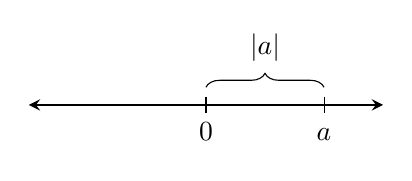
\begin{tikzpicture}[scale=1.5,decoration={brace,amplitude=5},text height=1.5ex,text depth=.25ex]
\draw [thick,stealth-stealth] (-1.5,0) -- (1.5,0);
\draw[shift={(0,0)},color=black] (0pt,2pt) -- (0pt,-2pt) node[below] {$0$};
\draw[shift={(1,0)},color=black] (0pt,2pt) -- (0pt,-2pt) node[below] {$a$};
\draw[decorate] (0,.15)--node[above=2.5mm]{$|a|$}(1,.15);
\end{tikzpicture}
}
\subcaptionbox{$a<0$\label{fig:distanceB}}[.48\linewidth]{
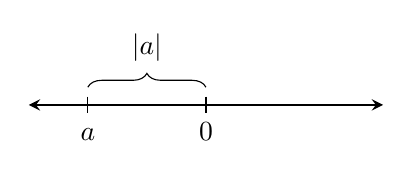
\begin{tikzpicture}[scale=1.5,decoration={brace,amplitude=5},text height=1.5ex,text depth=.25ex]
\draw [thick,stealth-stealth] (-1.5,0) -- (1.5,0);

\draw[shift={(0,0)},color=black] (0pt,2pt) -- (0pt,-2pt) node[below] {$0$};
\draw[shift={(-1,0)},color=black] (0pt,2pt) -- (0pt,-2pt) node[below] {$a$};
\draw[decorate] (-1,.15)--node[above=2.5mm]{$|a|$}(0,.15);

\end{tikzpicture}
}
\caption{Visual representation of $|a|$.}\label{fig:abs value as distance}
\end{figure}

\begin{theorem}
For all $a,b\in\mathbb{R}$, we have $|a-b|=|b-a|$. 
\end{theorem}

Given two points $a$ and $b$, $|a-b|$, and hence $|b-a|$ by the previous theorem, is the distance between $a$ and $b$ as shown in Figure~\ref{fig:distance between a and b}.

\begin{figure}[h!]
\centering
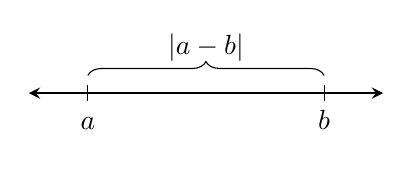
\begin{tikzpicture}[scale=1.5,decoration={brace,amplitude=5},text height=1.5ex,text depth=.25ex]
\draw [thick,stealth-stealth] (-1.5,0) -- (1.5,0);
\draw[shift={(-1,0)},color=black] (0pt,2pt) -- (0pt,-2pt) node[below] {$a$};
\draw[shift={(1,0)},color=black] (0pt,2pt) -- (0pt,-2pt) node[below] {$b$};
\draw[decorate] (-1,.15)--node[above=1mm]{$|a-b|$}(1,.15);
\end{tikzpicture}
\caption{Visual representation of $|a-b|$.}\label{fig:distance between a and b}
\end{figure}

\begin{theorem}
For all $a,b\in\mathbb{R}$, $|ab|=|a||b|$.
\end{theorem}

In the next theorem, writing $\pm a\leq b$ is an abbreviation for $a\leq b$ and $-a\leq b$.

\begin{theorem}
For all $a,b\in\mathbb{R}$, if $\pm a\leq b$, then $|a|\leq b$. 
\end{theorem}

\begin{theorem}
For all $a\in\mathbb{R}$, $|a|^2=a^2$.
\end{theorem}

\begin{theorem}\label{thm:plus minus less than or equal to abs value}
For all $a\in\mathbb{R}$, $\pm a\leq |a|$.
\end{theorem}

\begin{theorem}\label{thm:abs value less than or equal to iff squeezed by plus minus}
For all $a,r\in\mathbb{R}$ with $r$ nonnegative, $|a|\leq r$ if and only if $-r\leq a\leq r$.
\end{theorem}

%In the previous theorem, it must be the case that $r$ is nonnegative.  
The letter $r$ was used in the previous theorem because it is the first letter of the word ``radius". If $r$ is positive, we can think of the interval $(-r,r)$ as the interior of a one-dimensional circle with radius $r$ centered at 0. Figure~\ref{fig:abs value less than or equal to iff squeezed by plus minus} provides a visual interpretation of Theorem~\ref{thm:abs value less than or equal to iff squeezed by plus minus}.

\begin{figure}[h!]
\centering
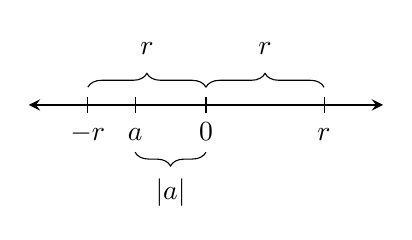
\begin{tikzpicture}[scale=1.5,decoration={brace,amplitude=5},text height=1.5ex,text depth=.25ex]
\draw [thick,stealth-stealth] (-1.5,0) -- (1.5,0);
\draw[shift={(0,0)},color=black] (0pt,2pt) -- (0pt,-2pt) node[below] {$0$};
\draw[shift={(1,0)},color=black] (0pt,2pt) -- (0pt,-2pt) node[below] {$r$};
\draw[shift={(-1,0)},color=black] (0pt,2pt) -- (0pt,-2pt) node[below] {$-r$};
\draw[shift={(-.6,0)},color=black] (0pt,2pt) -- (0pt,-2pt) node[below] {$a$};
\draw[decorate] (0,.15)--node[above=2.5mm]{$r$}(1,.15);
\draw[decorate] (-1,.15)--node[above=2.5mm]{$r$}(0,.15);
\draw[decorate] (0,-.4)--node[below=2.5mm]{$|a|$}(-.6,-.4);
\end{tikzpicture}
\caption{Visual representation of $|a|\leq r$.}\label{fig:abs value less than or equal to iff squeezed by plus minus}
\end{figure}

\begin{corollary}\label{cor:distance between two points less than or equal to}
For all $a,b,r\in\mathbb{R}$ with $r$ nonnegative, $|a-b|\leq r$ if and only if $b-r\leq a\leq b+r$.
\end{corollary}

Since $|a-b|$ represents the distance between $a$ and $b$, we can interpret $|a-b|\leq r$ as saying that the distance between $a$ and $b$ is less than or equal to $r$. In other words, $a$ is within $r$ units of $b$. See Figure~\ref{fig:visual of |a-b|<r}.

\begin{figure}[h!]
\centering
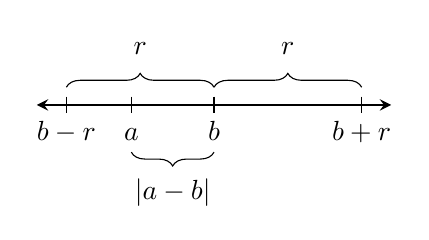
\begin{tikzpicture}[scale=1.5,decoration={brace,amplitude=5},text height=1.5ex,text depth=.25ex]
\draw [thick,stealth-stealth] (-1.5,0) -- (1.5,0);
\draw[shift={(0,0)},color=black] (0pt,2pt) -- (0pt,-2pt) node[below] {$b$};
\draw[shift={(1.25,0)},color=black] (0pt,2pt) -- (0pt,-2pt) node[below] {$b+r$};
\draw[shift={(-1.25,0)},color=black] (0pt,2pt) -- (0pt,-2pt) node[below] {$b-r$};
\draw[shift={(-.7,0)},color=black] (0pt,2pt) -- (0pt,-2pt) node[below] {$a$};
\draw[decorate] (0,.15)--node[above=2.5mm]{$r$}(1.25,.15);
\draw[decorate] (-1.25,.15)--node[above=2.5mm]{$r$}(0,.15);
\draw[decorate] (0,-.4)--node[below=2.5mm]{$|a-b|$}(-.7,-.4);
\end{tikzpicture}
\caption{Visual representation of $|a-b|\leq r$.}\label{fig:visual of |a-b|<r}
\end{figure}

Consider using Theorems~\ref{thm:plus minus less than or equal to abs value} and \ref{thm:abs value less than or equal to iff squeezed by plus minus} when attacking the next result, which is known as the \textbf{Triangle Inequality}.  This result can be extremely useful in some contexts. 

\begin{theorem}[Triangle Inequality]\label{thm:triangle inequality}
For all $a,b\in\mathbb{R}$, $|a+b|\leq |a|+|b|$.
\end{theorem}

Figure~\ref{fig:triangle inequality} depicts two of the cases for the Triangle Inequality.  

\begin{figure}[h!]
\centering
\subcaptionbox{$a\geq 0, b\geq 0$\label{fig:triangle A}}[.48\linewidth]{
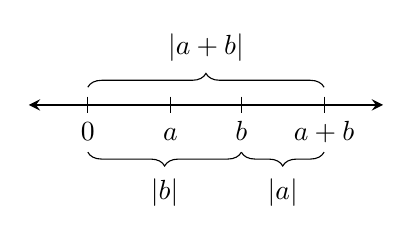
\begin{tikzpicture}[scale=1.5,decoration={brace,amplitude=5},text height=1.5ex,text depth=.25ex]
\draw [thick,stealth-stealth] (-1.5,0) -- (1.5,0);
\draw[shift={(-1,0)},color=black] (0pt,2pt) -- (0pt,-2pt) node[below] {$0$};
\draw[shift={(-.3,0)},color=black] (0pt,2pt) -- (0pt,-2pt) node[below] {$a$};
\draw[shift={(.3,0)},color=black] (0pt,2pt) -- (0pt,-2pt) node[below] {$b$};
\draw[shift={(1,0)},color=black] (0pt,2pt) -- (0pt,-2pt) node[below] {$a+b$};
\draw[decorate] (-1,.15)--node[above=2.5mm]{$|a+b|$}(1,.15);
\draw[decorate] (.3,-.4)--node[below=2.5mm]{$|b|$}(-1,-.4);
\draw[decorate] (1,-.4)--node[below=2.5mm]{$|a|$}(.3,-.4);
\end{tikzpicture}
}
\subcaptionbox{$a<0,b\geq 0$\label{fig:triangle B}}[.48\linewidth]{
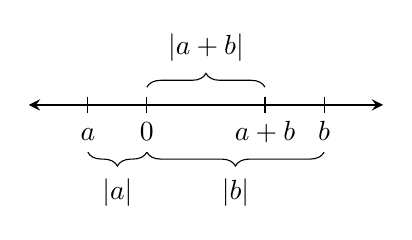
\begin{tikzpicture}[scale=1.5,decoration={brace,amplitude=5},text height=1.5ex,text depth=.25ex]
\draw [thick,stealth-stealth] (-1.5,0) -- (1.5,0);
\draw[shift={(-1,0)},color=black] (0pt,2pt) -- (0pt,-2pt) node[below] {$a$};
\draw[shift={(-.5,0)},color=black] (0pt,2pt) -- (0pt,-2pt) node[below] {$0$};
\draw[shift={(.5,0)},color=black] (0pt,2pt) -- (0pt,-2pt) node[below] {$a+b$};
\draw[shift={(1,0)},color=black] (0pt,2pt) -- (0pt,-2pt) node[below] {$b$};
\draw[decorate] (-.5,.15)--node[above=2.5mm]{$|a+b|$}(.5,.15);
\draw[decorate] (-.5,-.4)--node[below=2.5mm]{$|a|$}(-1,-.4);
\draw[decorate] (1,-.4)--node[below=2.5mm]{$|b|$}(-.5,-.4);
\end{tikzpicture}
}
\caption{Visual representation of two of the cases for the Triangle Inequality.}\label{fig:triangle inequality}
\end{figure}

\begin{problem}
Under what conditions do we have equality for the Triangle Inequality?
\end{problem}

Where did the Triangle Inequality get its name?  Why ``Triangle"?  For any triangle (including degenerate triangles), the sum of the lengths of any two sides must be greater than or equal to the length of the remaining side. That is, if $x$, $y$, and $z$ are the lengths of the sides of the triangle, then $z\leq x+y$, where we have equality only in the degenerate case of a triangle with no area. In linear algebra, the Triangle Inequality is a theorem about lengths of vectors. If $\mathbf{a}$ and $\mathbf{b}$ are vectors in $\mathbb{R}^n$, then the Triangle Inequality states that $\lVert \mathbf{a}+\mathbf{b}\rVert \leq \lVert\mathbf{a}\rVert +\lVert\mathbf{b}\rVert$. Note that $\lVert \mathbf{a}\rVert$ denotes the length of vector $\mathbf{a}$. See Figure~\ref{fig:triangle inequality 2d}. The version of the Triangle Inequality that we presented in Theorem~\ref{thm:triangle inequality} is precisely the one-dimensional version of the Triangle Inequality in terms of vectors.

\begin{figure}[h!]
\centering

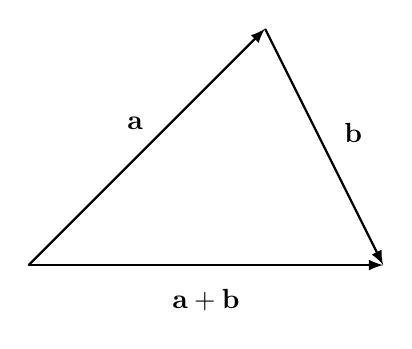
\begin{tikzpicture}[scale=1.5,text height=1.5ex,text depth=.25ex]
\coordinate (A) at (0,0) {};
\coordinate (B) at (3,0) {};
\coordinate (C) at (2,2) {};

\draw[thick, arrows={-latex}]  (A) -- (C) node[pos=0.45,above=2mm] {$\mathbf{a}$};
\draw[thick,arrows={-latex}]  (C) -- (B) node[pos=0.45,right=2mm] {$\mathbf{b}$};
\draw[thick, arrows={-latex},line cap=round]  (A) -- (B) node[midway,below=2mm] {$\mathbf{a}+\mathbf{b}$};
\end{tikzpicture}
\caption{Triangle Inequality in terms of vectors.}\label{fig:triangle inequality 2d}
\end{figure}

The next theorem is sometimes called the \textbf{Reverse Triangle Inequality}.

\begin{theorem}[Reverse Triangle Inequality]
For all $a,b\in\mathbb{R}$, $|a-b|\geq \left||a|-|b| \right|$.
\end{theorem}

Before we introduce the Completeness Axiom, we need some additional terminology.

\begin{definition}
Let $A\subseteq \mathbb{R}$. A point $b$ is called an \textbf{upper bound} of $A$ if for all $a\in A$, $a\leq b$. The set $A$ is said to be \textbf{bounded above} if it has an upper bound.
\end{definition}

\begin{problem}
The notion of a \textbf{lower bound} and the property of a set being \textbf{bounded below} are defined similarly. Try defining them.
\end{problem}

\begin{problem}\label{prob:find upper bounds}
Find all upper bounds and all lower bounds for each of the following sets when they exist.
\begin{enumerate}[label=\textrm{(\alph*)}]
\item $\{5,11,17,42,103\}$ 
\item $\mathbb{N}$
\item $\mathbb{Z}$
\item $(0,1]$
\item $(0,1]\cap \mathbb{Q}$
\item $(0,\infty)$
\item $\{42\}$
\item $\{\frac{1}{n}\mid n\in\mathbb{N}\}$
\item $\{\frac{1}{n}\mid n\in\mathbb{N}\}\cup\{0\}$
\item $\emptyset$
\end{enumerate}
\end{problem}

\begin{definition}
A set $A\subseteq \mathbb{R}$ is \textbf{bounded} if $A$ is bounded above and below.
\end{definition}

Notice that a set $A\subseteq\mathbb{R}$ is bounded if and only if it is a subset of some bounded closed interval.

\begin{definition}
Let $A\subseteq \mathbb{R}$. A point $p$ is a \textbf{supremum} (or \textbf{least upper bound}) of $A$ if $p$ is an upper bound of $A$ and $p\leq b$ for every upper bound $b$ of $A$.  Analogously, a point $p$ is an \textbf{infimum} (or \textbf{greatest lower bound}) of $A$ if $p$ is a lower bound of $A$ and $p\geq b$ for every lower bound $b$ of $A$. 
\end{definition}

Our next result tells us that a supremum of a set and an infimum of a set are unique when they exist.

\begin{theorem}
If $A\subseteq \mathbb{R}$ such that a supremum (respectively, infimum) of $A$ exists, then the supremum (respectively, infimum) of $A$ is unique.
\end{theorem}

In light of the previous theorem, if the supremum of $A$ exists, it is denoted by $\tcboxmath{\sup(A)}$. Similarly, if the infimum of $A$ exists, it is denoted by $\tcboxmath{\inf(A)}$. 

\begin{problem}
Find the supremum and the infimum of each of the sets in Problem~\ref{prob:find upper bounds} when they exist.
\end{problem}

It is important to recognize that the supremum or infimum of a set may or may not be contained in the set. In particular, we have the following theorem concerning suprema and maximums. The analogous result holds for infima and minimums.

\begin{theorem}
Let $A\subseteq \mathbb{R}$. Then $A$ has a maximum if and only if $A$ has a supremum and $\sup(A)\in A$, in which case the $\max(A)=\sup(A)$.
\end{theorem}

Intuitively, a point is the supremum of a set $A$ if and only if no point smaller than the supremum can be an upper bound of $A$. The next result makes this more precise.

\begin{theorem}\label{thm:scoot in characterization of sup}
Let $A\subseteq \mathbb{R}$ such that $A$ is bounded above and let $b$ be an upper bound of $A$. Then $b$ is the supremum of $A$ if and only if for every $\varepsilon >0$, there exists $a\in A$ such that $b-\varepsilon <a$.
\end{theorem}

\begin{problem}
State and prove the analogous result to Theorem~\ref{thm:scoot in characterization of sup} involving infimum.
\end{problem}

The following axiom states that every nonempty subset of the real numbers that has an upper bound has a least upper bound.

\begin{axiom}[Completeness Axiom]\label{axiom:completeness}
If $A$ is a nonempty subset of $\mathbb{R}$ that is bounded above, then $\sup(A)$ exists.
\end{axiom}

Given the Completeness Axiom, we say that the real numbers satisfy the \textbf{least upper bound property}. It is worth mentioning that we do not need the Completeness Axiom to conclude that every nonempty subset of the integers that is bounded above has a supremum, as this follows from Theorem~\ref{thm:reverse WOP} (a generalized version of the Well-Ordering Principle). 

Certainly, the real numbers also satisfy the analogous result involving infimum.

\begin{theorem}
If $A$ is a nonempty subset of $\mathbb{R}$ that is bounded below, then $\inf(A)$ exists.
\end{theorem}

Our next result, called the \textbf{Archimedean Property}, tells us that for every real number, we can always find a natural number that is larger. To prove this theorem, consider a proof by contradiction and then utilize the Completeness Axiom and Theorem~\ref{thm:scoot in characterization of sup}.

\begin{theorem}[Archimedean Property]
For every $x\in\mathbb{R}$, there exists $n\in\mathbb{N}$ such that $x<n$.
\end{theorem}

More generally, we can ``squeeze" every real number between a pair of integers. The next result is sometimes referred to at the \textbf{Generalized Archimedean Property}.

\begin{theorem}[Generalized Archimedean Property]
For every $x\in\mathbb{R}$, there exists $k,n\in\mathbb{Z}$ such that $k<x<n$.
\end{theorem}

\begin{theorem}\label{thm:small reciprocal}
For any positive real number $x$, there exists $N\in \mathbb{N}$ such that $0<\frac{1}{N}<x$.
\end{theorem}

The next theorem strengthens the Generalized Archimedean Property and says that every real number is either an integer or lies between a pair of consecutive integers. To prove this theorem, let $x\in\mathbb{R}$ and define $L=\{k\in\mathbb{Z}\mid k\leq x\}$. Use the Generalized Archimedean Property to conclude that $L$ is nonempty and then utilize Theorem~\ref{thm:reverse WOP}.

\begin{theorem}\label{thm:squeeze with consecutive integers}
For every $x\in\mathbb{R}$, there exists $n\in \mathbb{Z}$ such that $n\leq x<n+1$.
\end{theorem}

To prove the next theorem, let $a<b$, utilize Theorem~\ref{thm:small reciprocal} on $b-a$ to obtain $N\in\mathbb{N}$ such that $\frac{1}{N}<b-a$, and then apply Theorem~\ref{thm:squeeze with consecutive integers} to $Na$ to conclude that there exists $n\in\mathbb{N}$ such that $n\leq Na<n+1$. Lastly, argue that $\frac{n+1}{N}$ is the rational number you seek.

\begin{theorem}\label{thm:rationals dense}
If $(a,b)$ is an open interval, then there exists a rational number $p$ such that $p\in(a,b)$.
\end{theorem}

Recall that the real numbers consist of rational and irrational numbers.  Two examples of an irrational number that you are likely familiar with are $\pi$ and  $\sqrt{2}$. In Section~\ref{sec:Irrationality_of_Root_2}, we will prove that $\sqrt{2}$ is irrational, but for now we will take this fact for granted. It turns out that $\sqrt{2}\approx 1.41421356237\in (1,2)$. This provides an example of an irrational number occurring between a pair of distinct rational numbers. The following theorem is a good challenge to generalize this.

\begin{theorem}\label{thm:irrationals dense}
If $(a,b)$ is an open interval, then there exists an irrational number $p$ such that $p\in(a,b)$.
\end{theorem}

Repeated applications of the previous two theorems implies that every open interval contains infinitely many rational numbers and infinitely many irrational numbers. In light of these two theorems, we say that both the rationals and irrationals are \textbf{dense} in the real numbers. 

\epigraph{If people do not believe that mathematics is simple, it is only because they do not realize how complicated life is.}{John von Neumann, mathematician}
\end{section}